\documentclass{article}
\usepackage{graphicx}
\usepackage{textcomp}
\usepackage{amssymb}

\title{Redes Neurais}
\author{Augusto Rodrigo Camblor Santos }
\date{02/06/ 2023}

\begin{document}

\maketitle

\section{Descrição}

\begin{flushleft}
Este projeto tem como base um estudo sobre redes neurais, onde será utilizado um código base fornecido em aula pelo professor ministrador do curso de cálculo.
\end{flushleft}
\begin{flushleft}
Neste projeto, a finalidade é um estudo prático onde ocorre uma classificação através de entradas no console; as três primeiras entradas correspondem às entradas dos pesos denominados como $W$, na sequência há mais três entradas que correspondem ao bias denominadas como $B$, por fim as duas últimas entradas são determinadas por \textit{learning rate} ($lr$) e a taxa de aprendizagem de erro (\textit{err}). A partir disso, há uma captação dos valores do gradiente que resultará em um treinamento para classificar se um número é primo ou não, e se ele é par ou ímpar.
\end{flushleft}

\section{O que eu quero Classificar}

\textbf{Número Pares e Ímpares}

\begin{flushleft}
No livro de \textit{Fundamentos da Matemática Elementar} volume 1 do Gelson Iezzi:
\end{flushleft}

\begin{quote}
    \setlength{\parindent}{4cm}
    \setlength{\baselineskip}{1.5\baselineskip}
    \fontsize{10}{10}\selectfont
    "Quando $a$ é divisor de $b$, dizemos que '$b$ é divisível por $a$' ou '$b$ é múltiplo de $a$'."
\end{quote}
\begin{quote}
    \setlength{\parindent}{4cm}
    \setlength{\baselineskip}{1.5\baselineskip}
    \fontsize{10}{10}\selectfont
    "Para um inteiro $a$ qualquer, indicamos com $D(a)$ o conjunto de seus divisores e com $M(a)$ o conjunto de seus múltiplos."(Iezzi, p.~43)\cite{iezzifundamentos}
\end{quote}


\begin{flushleft}
Com esse fundamento, a classificação dos números pares ou ímpares é determinada pela divisibilidade por 2. Segundo Carl Friedrich Gauss: ``Um número é par se for divisível por 2, e ímpar caso contrário". Portanto, ao realizar a divisão e o número do resultado for um número inteiro, a classificação é par; caso contrário, a classificação é ímpar. E de acordo com o matemático francês Évariste Galois: ``Os números pares são como soldados, marchando em pares e facilmente alinhados. Os números ímpares são como artistas temperamentais, nunca se encaixando perfeitamente".
\end{flushleft}
\newpage
\begin{flushleft}
Exemplos dos números pares:
\end{flushleft}

\begin{itemize}
  \item $4 \div 2 = 2$ (resultado inteiro, portanto 4 é par)
  \item $10 \div 2 = 5$ (resultado inteiro, portanto 10 é par)
\end{itemize}

\begin{flushleft}
Exemplos dos números ímpares:
\end{flushleft}

\begin{itemize}
  \item $7 \div 2 = 3.5$ (resultado não inteiro, portanto 7 é ímpar)
  \item $15 \div 2 = 7.5$ (resultado não inteiro, portanto 15 é ímpar)
\end{itemize}

\begin{flushleft}
A expressão algébrica que comprova as afirmações e citações anteriores:
\end{flushleft}

\begin{itemize}
  \item $2n + 1$ para números ímpares
  \item $2n$ para números pares
\end{itemize}
\begin{flushleft}
Em suma, a divisibilidade por 2 é o critério principal para classificar um número como par ou ímpar. Essa distinção é essencial na estruturação dos números inteiros, permitindo a compreensão e manipulação dos padrões numéricos. Portanto, no código feito para o treinamento, não valida números negativos por não fazerem parte do conjunto, sendo assim, a resposta retornada no console para casos numéricos negativos será "False".
\end{flushleft}

\textbf{Números Primos}

\begin{flushleft}
Um número é considerado primo se ele possui exatamente dois divisores, sendo o 1 e ele mesmo. Em outras palavras, um número primo é um número inteiro maior que 1 que não pode ser dividido de forma exata por nenhum outro número além de ele mesmo e pelo 1.
\end{flushleft}

\begin{flushleft}
Outro meio de encontrar um número primo é utilizando o método da divisão por todos os números inteiros menores que ele mesmo, até a raiz quadrada desse número. Se nenhum desses números for um divisor exato, então o número é primo. Com exceção do número 2, por ser o único número par que é primo, é possível fazer uma verificação separada para ele e, em seguida, aplicar o método da divisão para os demais números ímpares.
\end{flushleft}

\begin{flushleft}
Segundo Gauss, "Os números primos são os indivíduos solitários do reino dos números, sem divisores além de si mesmos e da unidade". Ressaltando que a verificação dessa classificação se torna mais eficiente para números grandes utilizando algoritmos mais avançados, como Crivo de Eratóstenes ou o teste de primalidade de Miller-Rabin.
\end{flushleft}

\begin{flushleft}
No livro de \textit{Fundamentos da Matemática Elementar} volume 1 do Gelson Iezzi:
\end{flushleft}

\begin{quote}
    \setlength{\parindent}{4cm}
    \setlength{\baselineskip}{1.5\baselineskip}
    \fontsize{10}{10}\selectfont
    "Uma importante noção que devemos ter sobre números inteiros é o conceito de divisor".
\end{quote}

\newpage

\begin{quote}
    \setlength{\parindent}{4cm}
    \setlength{\baselineskip}{1.5\baselineskip}
    \fontsize{10}{10}\selectfont
    "Dizemos que o inteiro $a$ é divisor do inteiro $b$ (símbolo $a|b$) quando existe um inteiro $c$ tal que $ca = b$." (Iezzi, p.~43)\cite{iezzifundamentos}
\end{quote}

\begin{flushleft}
Nos trazendo a expressão algébrica:
\end{flushleft}

$a\,|\,b \Leftrightarrow (\,\exists\, \,c\, \in \mathbb{Z} \,|\, ca = b)$.

\begin{flushleft}
Exemplos de números primos e seus casos:
\end{flushleft}
\begin{itemize}
  \item O número 2 é o único número primo par, pois só é divisível por 1 e 2.
  \item O número 3 também é primo, pois só é divisível por 1 e 3.
  \item O número 4 não é primo, pois além de ser divisível por 1 e 4, também é divisível por 2.
\end{itemize}

\begin{flushleft}
Em resumo, os números primos são elementos fundamentais na estrutura dos números e possuem propriedades únicas que os diferenciam dos demais.
\end{flushleft}

\newpage

\section{Função de Erro}
\begin{flushleft}
Abaixo uma imagem da qual representa a função erro e a equação y feitas a mão, dentro do código a função erro pode ser encontrada como 'errnovo' dentro da função '\textit{ def descentV }'.
\end{flushleft}

\begin{flushleft}
A tolerância feita no código foi de: $10^{-6}$, encontrada no código como '\textit{tol}' dentro '\textit{ descentV }' também.
\end{flushleft}

\begin{flushleft}
No código a equação $\hat{y}_\textsubscript{i}$ pode ser encontrada na função '\textit{ predict }' em seu retorno.
\end{flushleft}

\begin{figure}[htbp]
    \centering
    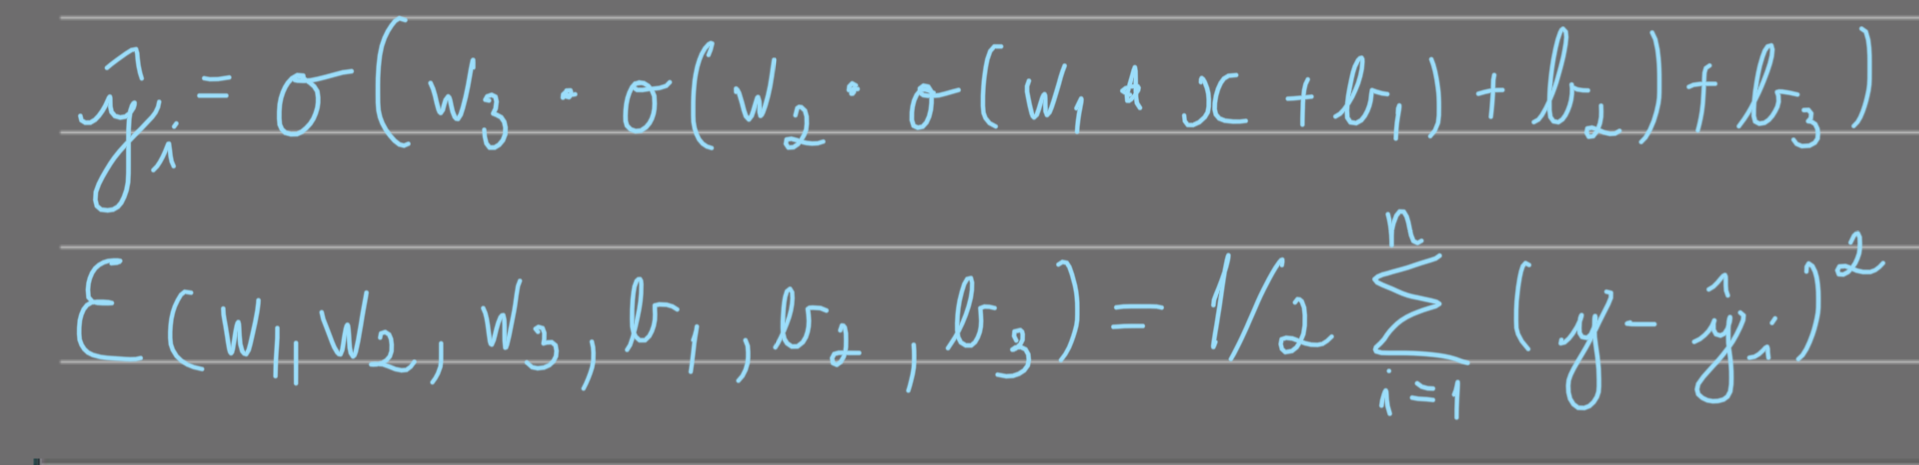
\includegraphics[width=0.8\textwidth]{Funcao_Erro e Funcao y.png}
    \caption{Ilustra a função "erro" e a equação $\hat{y}_\textsubscript{i}$ feitas a mão}
    \label{fig:funcao_erro1}
\end{figure}

\begin{figure}[htbp]
    \centering
    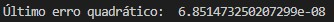
\includegraphics[width=0.8\textwidth]{Ultimo Erro Quadratico.jpg}
    \caption{Último erro quadrático}
    \label{fig:funcao_erro2}
\end{figure}

\newpage

\section{Sigmoide}
\begin{flushleft}
Abaixo seguem dois exemplos de sigmoide. O primeiro ilustra como a função geradora do gráfico está funcionando com valores que geram grau de significância para a sigmoide. Já o segundo exemplo é uma 'plotagem' da sigmoide com os valores utilizados como exemplos citados mais abaixo no relatório. A função referida no código é encontrada em duas etapas. 
\end{flushleft}

\begin{flushleft}
A função que realiza o cáculo se chama '\textit{ sigmoid }'. Já a função que realiza a 'plotagem' do gráfico se chama '\textit{plot\_sigmoid}'.
\end{flushleft}

\begin{figure}[htbp]
    \centering
    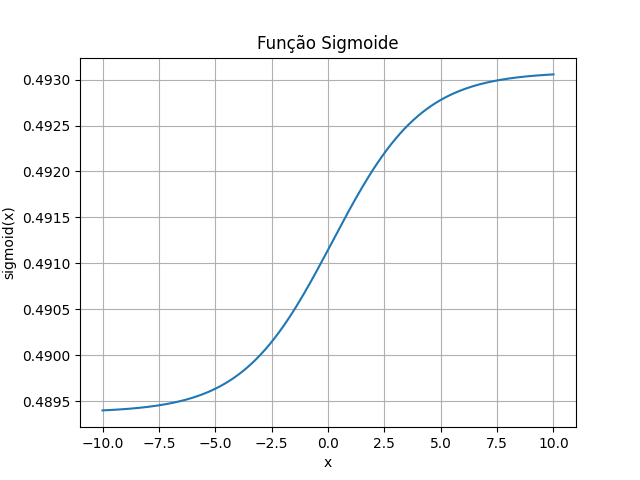
\includegraphics[width=0.8\textwidth]{Figure_2.png}
    \caption{Sigmoide com valores de pesos e bias definidos}
    \label{fig:sigmoide1}
\end{figure}


\begin{figure}
    \centering
    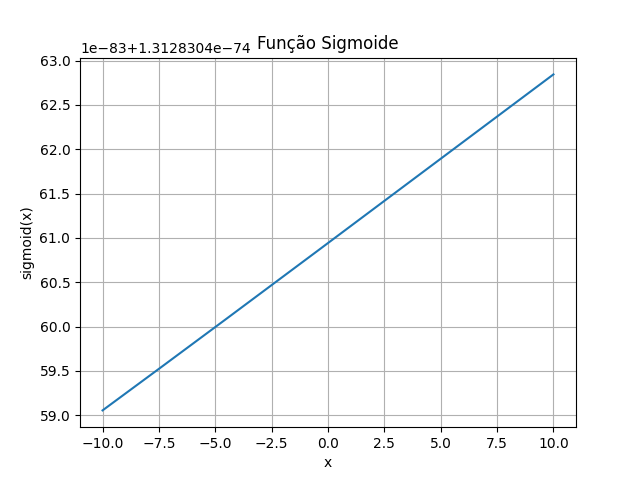
\includegraphics[width=0.8\textwidth]{Figure_3.png}
    \caption{Sigmoide com valores não definidos}
    \label{fig:sigmoide2}
\end{figure}
\newpage

\section{Gradiente}

\begin{flushleft}
Abaixo há a plotagem do gráfico do gradiente dos valores exemplos. A função no código pode ser encontrada em duas etapas. A que realiza o cálculo se chama '\textit{ descentV }'. Já a função que realiza a criação do gráfico se chama '\textit{plot\_gradient}'.
\end{flushleft}

\begin{flushleft}
A função que realiza o gráfico é acompanhada das e chamada após o cálculo feita na função '\textit{ neural } que utiliza as derivadas da função $\hat{y}_\textsubscript{i}$.
\end{flushleft}

\newpage
\begin{figure}
  \centering
  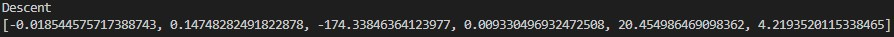
\includegraphics[width=0.8\textwidth]{Descent.jpg}
  \caption{Valores do gradiente}
  \label{fig:gradiente1}
\end{figure}
\newpage

\begin{figure}
  \centering
  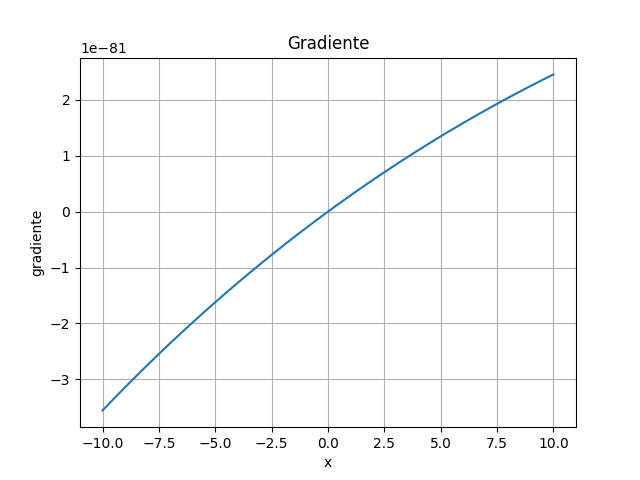
\includegraphics[width=0.8\textwidth]{Figure_1.png}
  \caption{Gradiente dos valores informados}
  \label{fig:gradiente2}
\end{figure}

\newpage

\subsection{Derivadas dos pesos e bias feitas a mão}
\begin{flushleft}
Calculo das derividas dos pesos feitos a mão
\end{flushleft}

\begin{figure}
  \centering
  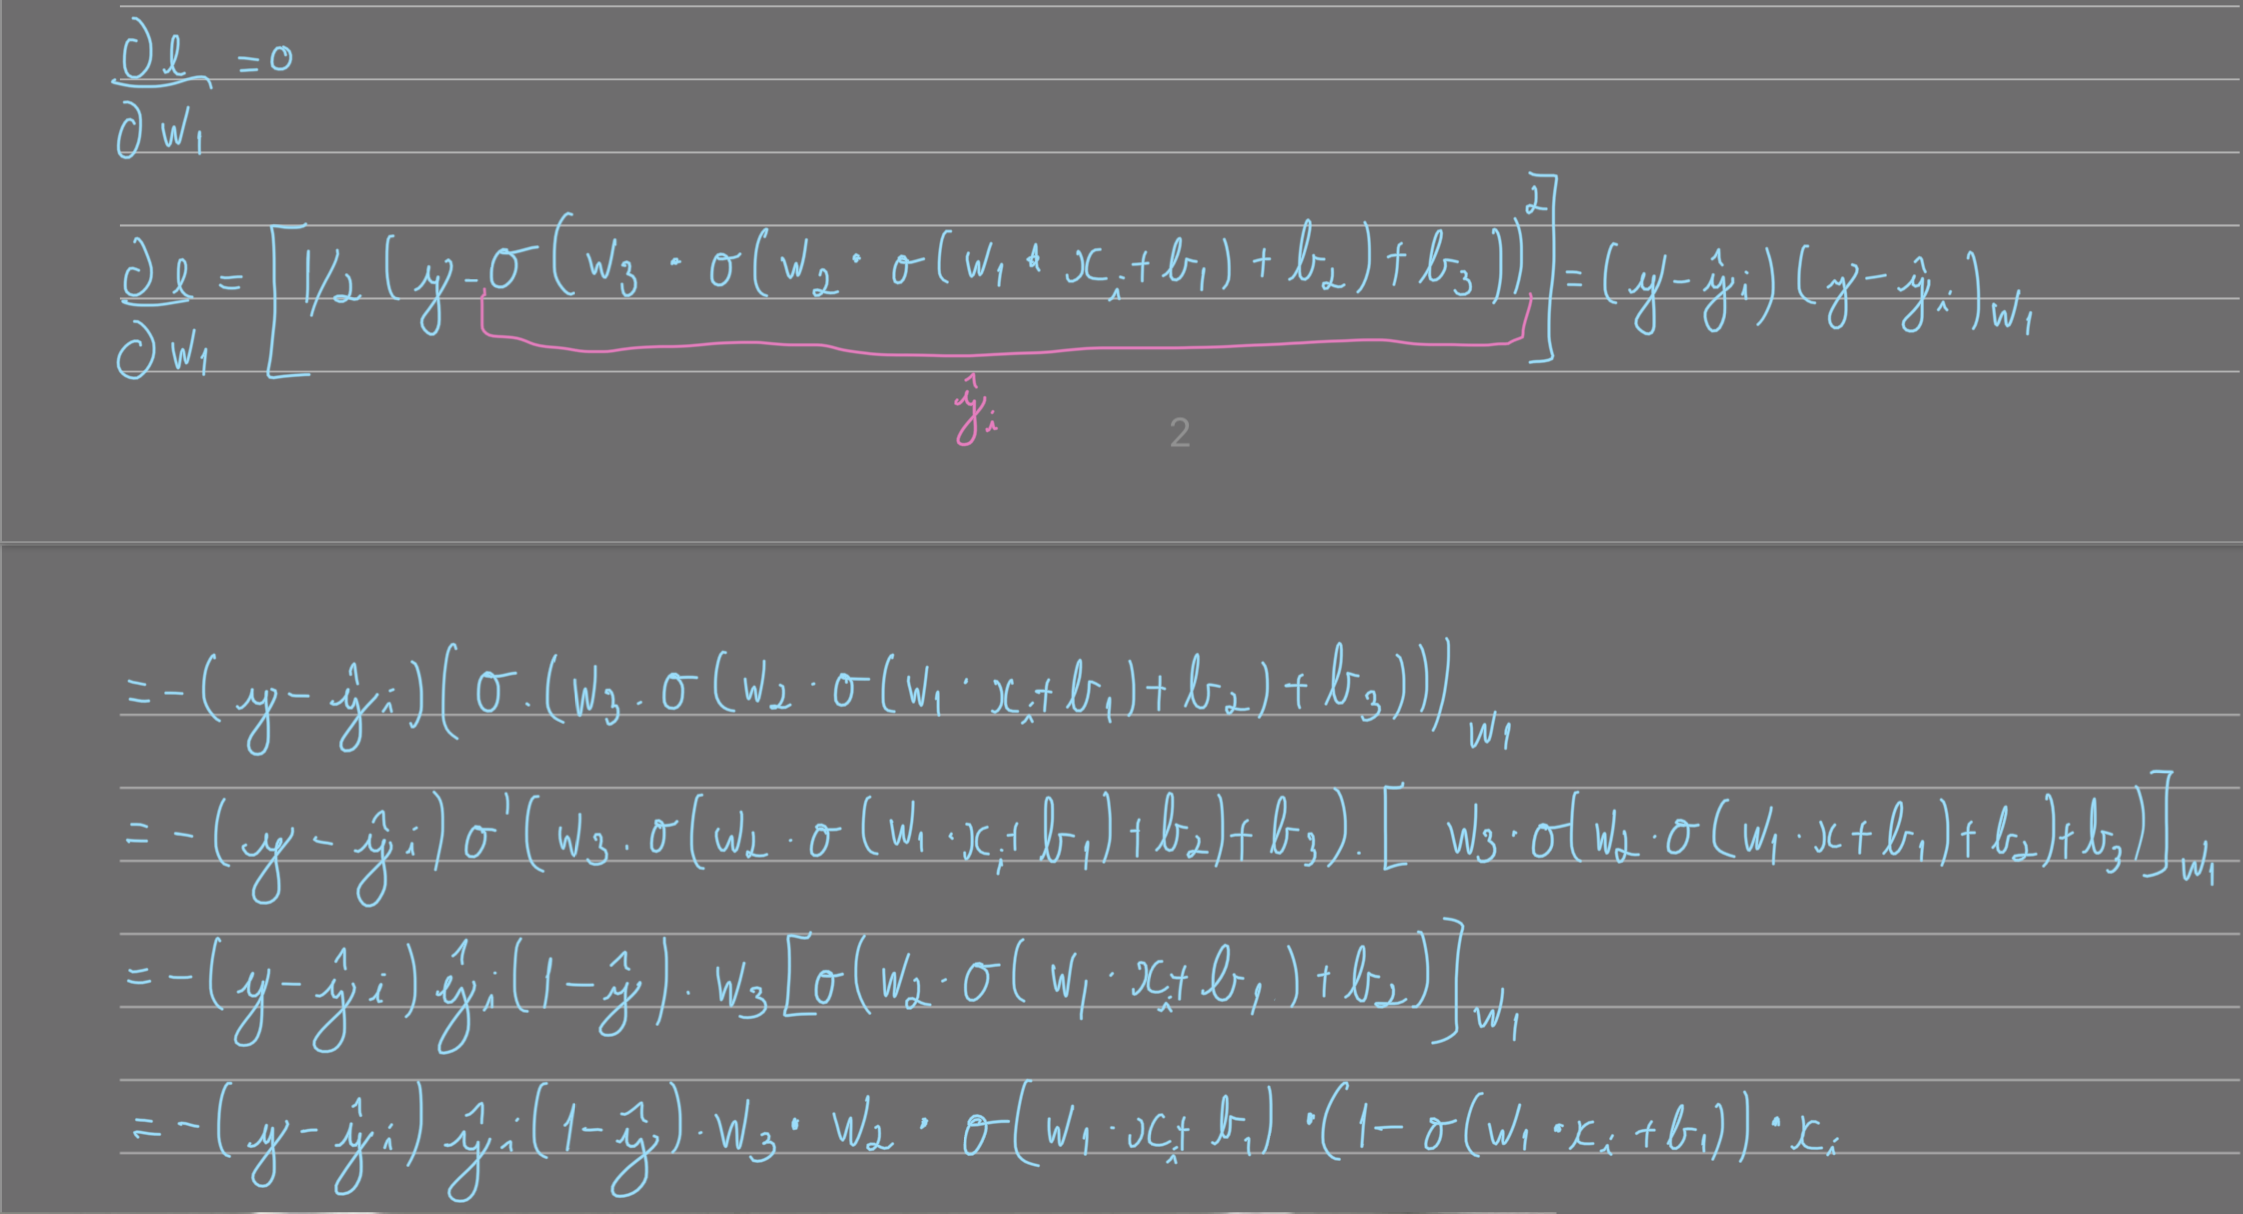
\includegraphics[width=0.8\textwidth]{Derivada_w1.png}
  \caption{Derivada w1}
  \label{fig:gradiente3}
\end{figure}

\begin{figure}
  \centering
  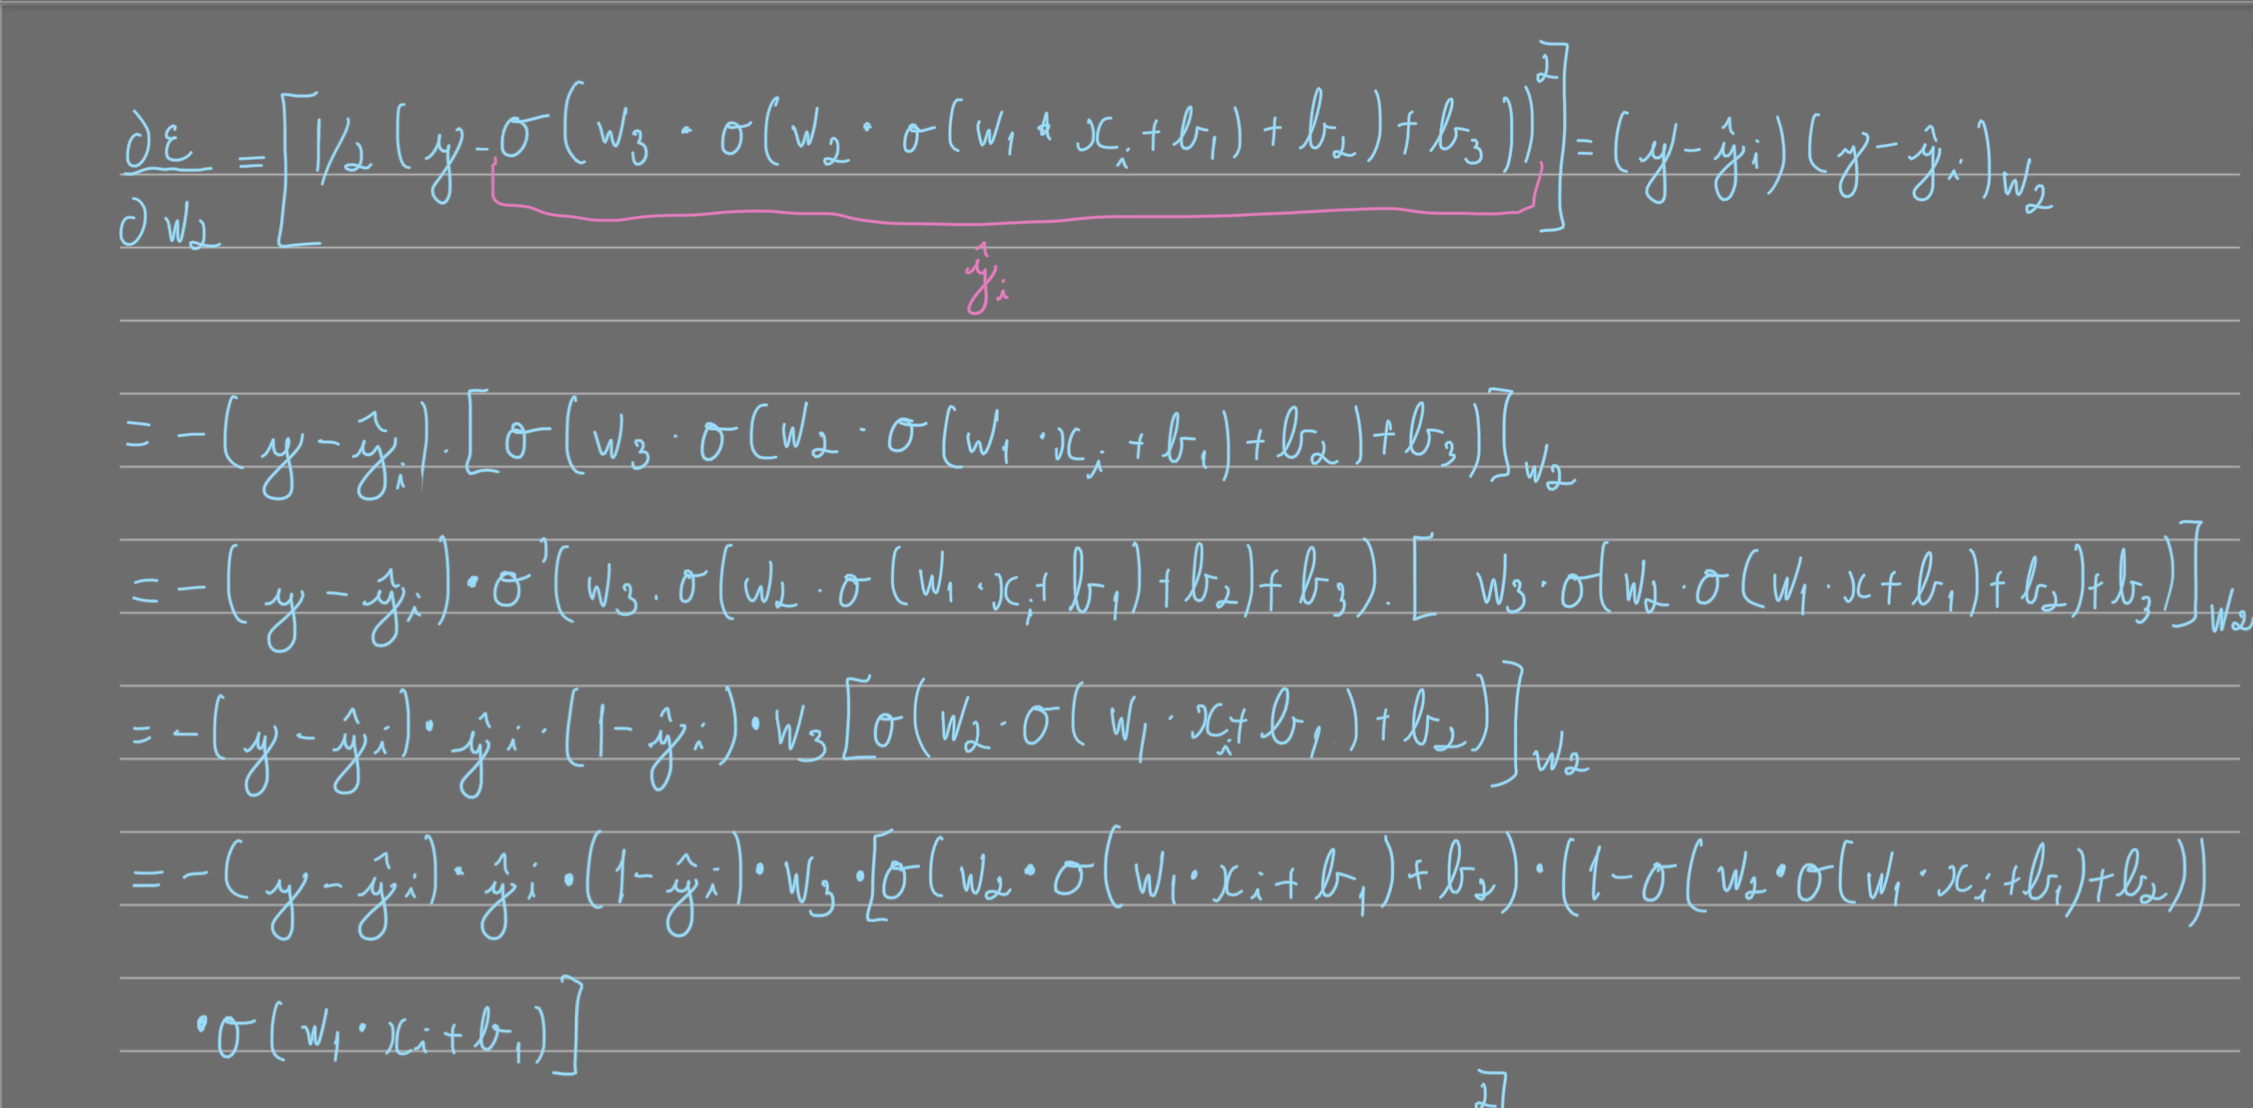
\includegraphics[width=0.8\textwidth]{Derivada_w2.png}
  \caption{Derivada w2}
  \label{fig:gradiente4}
\end{figure}

\begin{figure}
  \centering
  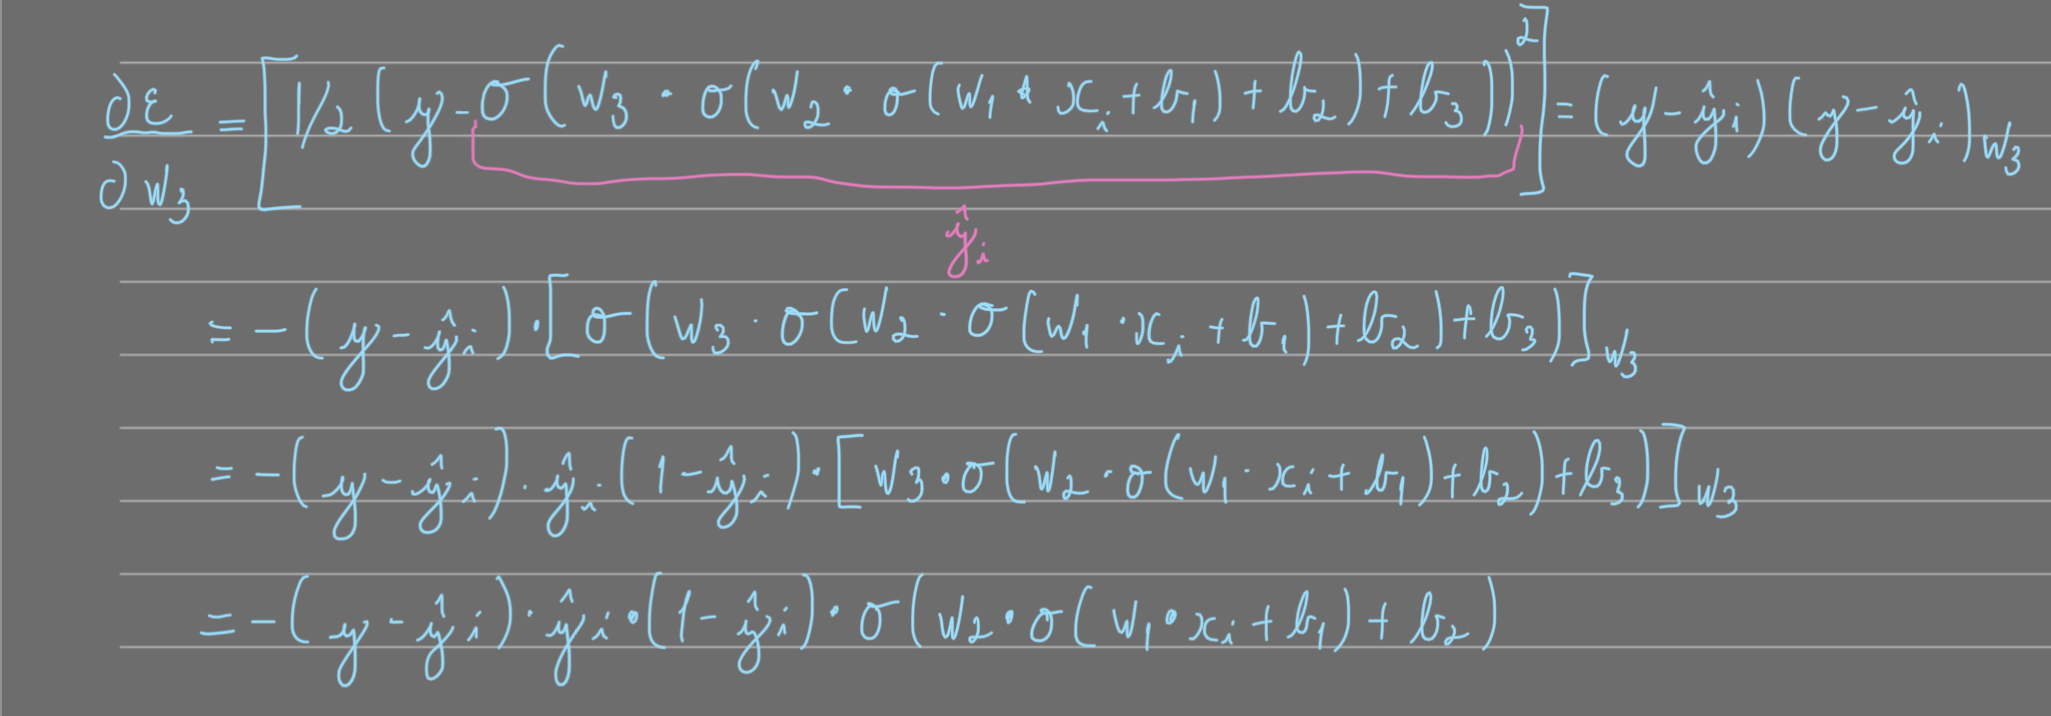
\includegraphics[width=0.8\textwidth]{Derivada_w3.png}
  \caption{Derivada w3}
  \label{fig:gradiente5}
\end{figure}

\begin{figure}
  \centering
  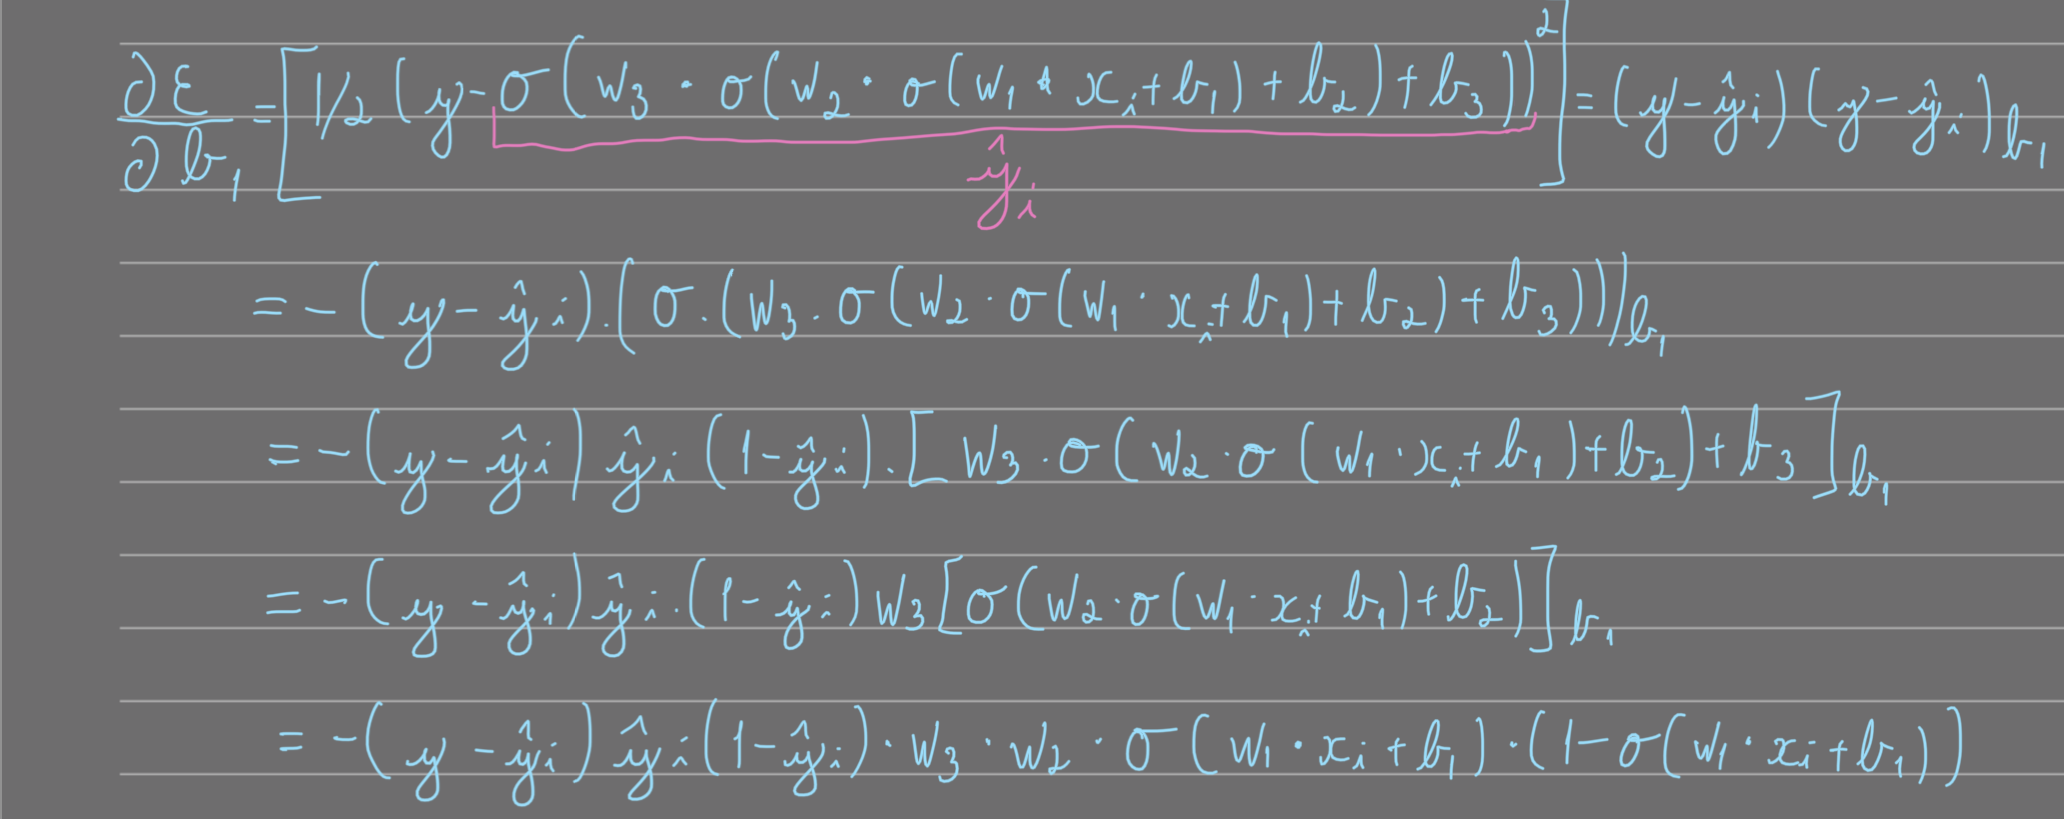
\includegraphics[width=0.8\textwidth]{Derivada_b1.png}
  \caption{Derivada b1}
  \label{fig:gradiente6}
\end{figure}

\begin{figure}
  \centering
  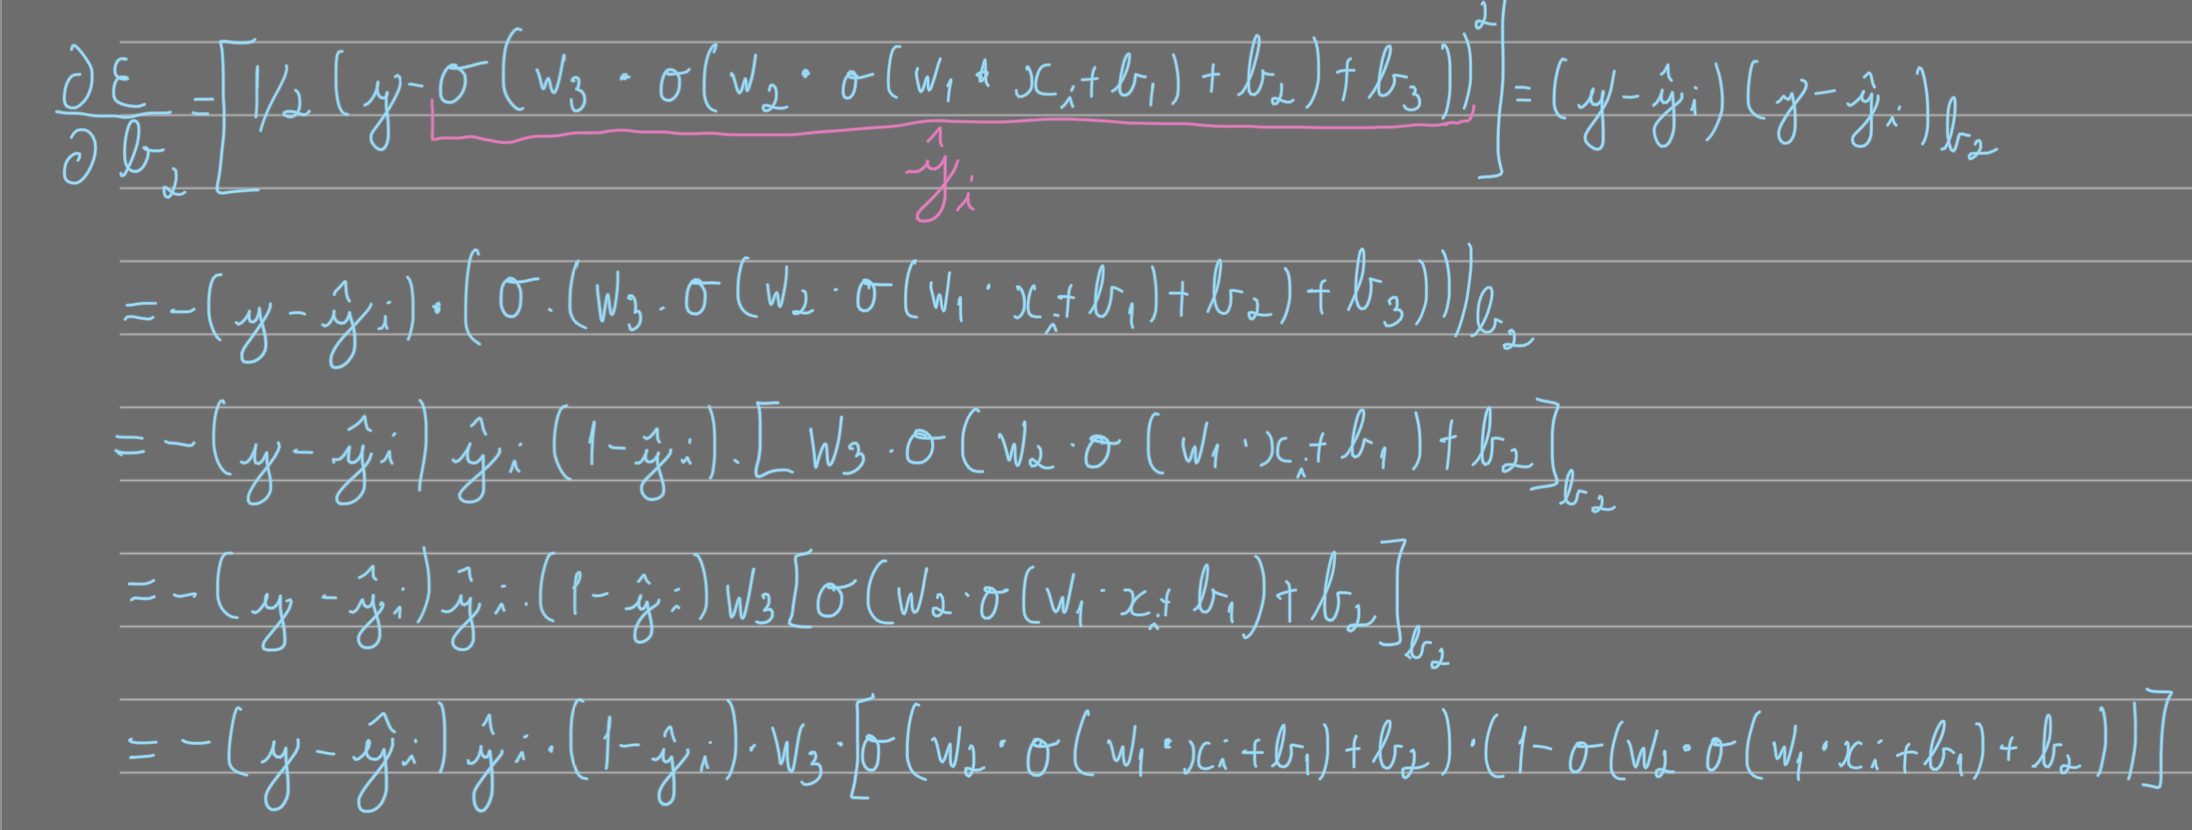
\includegraphics[width=0.8\textwidth]{Derivada_b2.png}
  \caption{Derivada b2}
  \label{fig:gradiente7}
\end{figure}

\begin{figure}
  \centering
  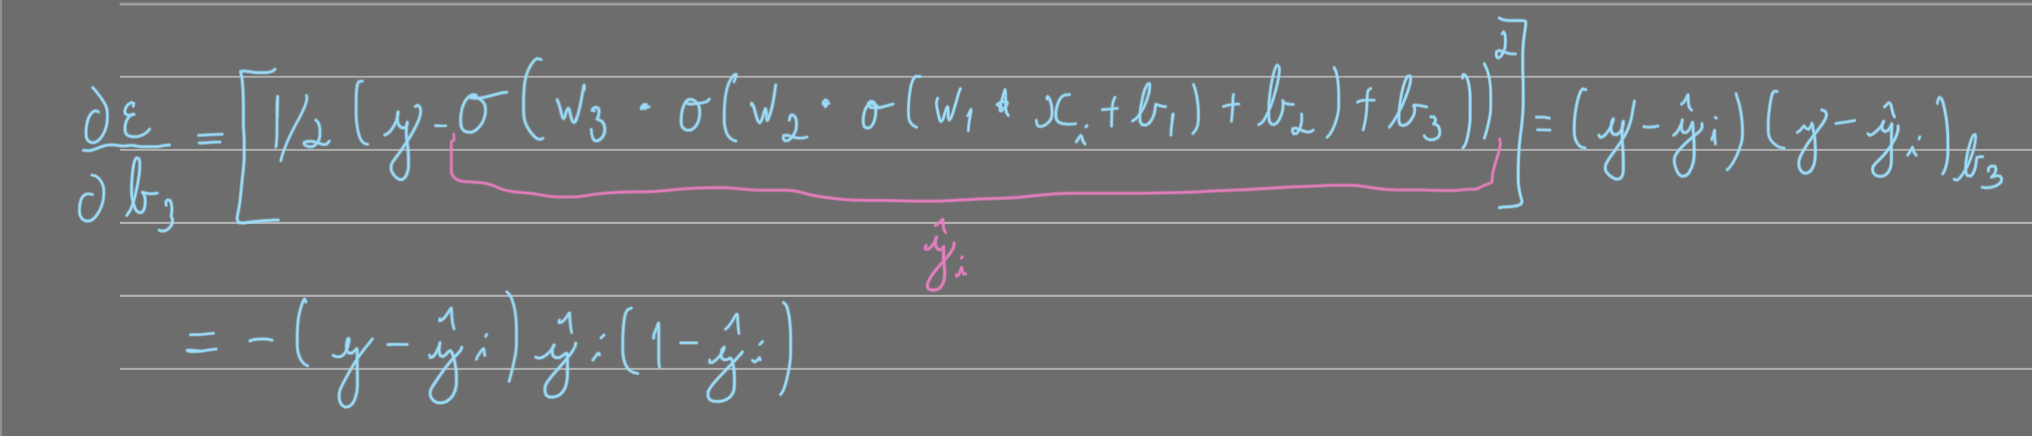
\includegraphics[width=0.8\textwidth]{Derivada_b3.png}
  \caption{Derivada b3}
  \label{fig:gradiente8}
\end{figure}
\newpage

\newpage

\section{Parâmetros de Teste}
\begin{flushleft}
Os valores utilizados para $w_1$, $w_2$, $w_3$, $b_1$, $b_2$, $b_3$, taxa de aprendizado (lr) e erro foram:
\end{flushleft}

\begin{itemize}
  \item $w_1 = 0.05$
  \item $w_2 = 0.07$
  \item $w_3 = 0.03$
  \item $b_1 = -0.02$
  \item $b_2 = 0.01$
  \item $b_3 = -0.03$
  \item $lr = 0.1$
  \item $err = 0.001$
\end{itemize}

\newpage
\section{Conclusões}

\begin{flushleft}
Dos resultados obtidos é possivel ver que o treinamento foi realizado e predição da rede neural atua, com isso classificando os números como primos ou não e pares ou ímpares, como os exemplos abaixo:
\end{flushleft}

\newpage

\begin{figure}
    \centering
    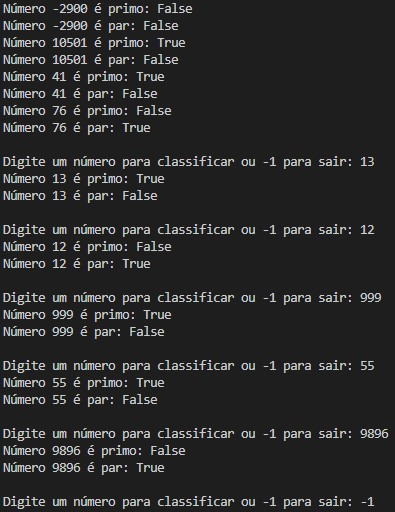
\includegraphics[width=0.8\textwidth]{Exemplos_2.jpg}
    \caption{Exemplos de respostas}
    \label{fig:conclusões}
\end{figure}

\section{Link do GitHub}

Insira aqui o link do GitHub do projeto.
\newpage
\begin{thebibliography}{9}
  \bibitem{iezzifundamentos} 
  Iezzi, Gelson. \textit{Fundamentos da Matemática Elementar}, volume 1.
\end{thebibliography}

\end{document}